\documentclass[sigconf]{acmart}

\usepackage{booktabs} % For formal tables
\hypersetup{colorlinks,
  urlcolor=[rgb]{0.5,0.5,0.5},
            %citecolor=[rgb]{0.5,0.5,0.5},
            citecolor=blue,
            linkcolor=blue}
\usepackage{enumerate}


% Copyright
%\setcopyright{none}
%\setcopyright{acmcopyright}
%\setcopyright{acmlicensed}
\setcopyright{rightsretained}
%\setcopyright{usgov}
%\setcopyright{usgovmixed}
%\setcopyright{cagov}
%\setcopyright{cagovmixed}


%% DOI
%\acmDOI{10.475/123_4}
%
%% ISBN
%\acmISBN{123-4567-24-567/08/06}
%
%%Conference
\acmConference[CIKM'17]{ACM Conference on Information and Knowledge Management}{November 2017}{Singapore}
%\acmYear{1997}
%\copyrightyear{2016}
%
%\acmPrice{15.00}


\begin{document}
\title{RiskFinder: A Sentence-level Financial Risk Detector for Financial Reports}
%\titlenote{Produces the permission block, and
  %copyright information}
%\subtitle{Extended Abstract}
%\subtitlenote{The full version of the author's guide is available as
%  \texttt{acmart.pdf} document}

  \author{}
%\author{Yu-Wen Liu}
%%\authornote{Dr.~Trovato insisted his name be first.}
%%\orcid{1234-5678-9012}
%\affiliation{%
  %\institution{Department of Computer Science}
  %\streetaddress{National Chengchi University}
  %\city{Taipei}
  %%\state{Ohio}
  %\postcode{11605}
  %\country{Taiwan}
%}
%\email{g10435@cs.nccu.edu.tw}

%\author{Liang-Chih Liu}
%%\authornote{The secretary disavows any knowledge of this author's actions.}
%\affiliation{%
  %\institution{Department of Information Management and Finance}
  %\streetaddress{National Chiao Tung University}
  %\city{Hsinchu}
  %%\state{Ohio}
  %\postcode{30010}
  %\country{Taiwan}
%}
%\email{tony919kimo@nctu.edu.tw}

%\author{Chuan-Ju Wang}
%%\authornote{This author is the
%%  one who did all the really hard work.}
%\affiliation{%
  %\institution{Research Center of Information Technology Innovation}
  %\streetaddress{Academia Sinica}
  %\city{Taipei}
  %\postcode{11574}
  %\country{Taiwan}
%}
%\email{cjwang@citi.sinica.edu.tw}

%\author{Ming-Feng Tsai}
%\affiliation{
  %\institution{Department of Computer Science}
  %\streetaddress{National Chengchi University}
  %\city{Taipei}
  %\postcode{11605}
  %\country{Taiwan}
%}
%\email{mftsai@cs.nccu.edu.tw}

%\author{Sean Fogarty}
%\affiliation{%
%  \institution{NASA Ames Research Center}
%  \city{Moffett Field}
%  \state{California}
%  \postcode{94035}}
%\email{fogartys@amesres.org}
%
%\author{Charles Palmer}
%\affiliation{%
%  \institution{Palmer Research Laboratories}
%  \streetaddress{8600 Datapoint Drive}
%  \city{San Antonio}
%  \state{Texas}
%  \postcode{78229}}
%\email{cpalmer@prl.com}

%\author{John Smith}
%\affiliation{\institution{The Th{\o}rv{\"a}ld Group}}
%\email{jsmith@affiliation.org}

%\author{Julius P.~Kumquat}
%\affiliation{\institution{The Kumquat Consortium}}
%\email{jpkumquat@consortium.net}

% The default list of authors is too long for headers}
%\renewcommand{\shortauthors}{B. Trovato et al.}


\begin{abstract}
This paper demonstrates RiskFinder, a web-based information system for
facilitating the analyses of soft and hard information in financial reports.
In particular, the system broadens analysis from the word level to the
sentence level; this is novel in practitioner communities and
unprecedented among financial academics.
The proposed system has four main components: 1) a Form 10-K risk-sentiment
dataset, consisting of a set of labeled financial sentences and pre-trained
sentence embeddings; 2) metadata, including basic information on each
company that published the Form 10-K financial report as well as some relevant
financial measures; 3) an interface that highlights risk-related sentences in
the financial reports based on several sentence embedding techniques; 4) a
visualization of financial time-series data for the corresponding company.
This system considerably facilitates case studies in the field of finance and
can be of great help in capturing valuable insight within large amounts of
textual information.
\end{abstract}

%
% The code below should be generated by the tool at
% http://dl.acm.org/ccs.cfm
% Please copy and paste the code instead of the example below.
%
%\begin{CCSXML}
%<ccs2012>
% <concept>
%  <concept_id>10010520.10010553.10010562</concept_id>
%  <concept_desc>Computer systems organization~Embedded systems</concept_desc>
%  <concept_significance>500</concept_significance>
% </concept>
% <concept>
%  <concept_id>10010520.10010575.10010755</concept_id>
%  <concept_desc>Computer systems organization~Redundancy</concept_desc>
%  <concept_significance>300</concept_significance>
% </concept>
% <concept>
%  <concept_id>10010520.10010553.10010554</concept_id>
%  <concept_desc>Computer systems organization~Robotics</concept_desc>
%  <concept_significance>100</concept_significance>
% </concept>
% <concept>
%  <concept_id>10003033.10003083.10003095</concept_id>
%  <concept_desc>Networks~Network reliability</concept_desc>
%  <concept_significance>100</concept_significance>
% </concept>
%</ccs2012>
%\end{CCSXML}

%\ccsdesc[500]{Computer systems organization~Embedded systems}
%\ccsdesc[300]{Computer systems organization~Redundancy}
%\ccsdesc{Computer systems organization~Robotics}
%\ccsdesc[100]{Networks~Network reliability}
\keywords{financial risk, text mining, Form 10-K}

\maketitle


\section{Introduction}

A great deal of mass media outlets such as newspapers and magazines, or financial
report disclosures required by authorities such as the SEC\footnote{SEC indicates
Securities and Exchange Commission}-mandated Form-10Q and Form-10K, play an
important role in disseminating information to participants in financial
markets.
The spread of this information may quickly or slowly influence the sentiment of 
market participants and thus reshape their perspectives on economic
numbers, such as stock prices and interest rate levels.
This information comes in two types: soft information, usually
referring to textual information such as opinions, ideas, and market
commentary; and hard information, that is, numerical information such as historical
time series of stock prices.

Due to the strong relation between the textual information and numerical
measures, there have been a growing body of studies in the fields of finance
and data science that adopt the techniques of natural language processing (NLP) and
machine learning to examine the interaction between these two types of
information~\citep[e.g.,][]{loughran2016textual,kogan2009predicting,tsai2017risk,Tsai:2016:DFK:2991040.2948072,rekabsaz2017volatility,agarwal2016information,tsai2016impact}.
For example, these
studies~\citep{loughran2011liability,campbell2014information,jegadeesh2013word}
investigate how the disclosures of finance sentiment or risk keywords in
SEC-mandated financial reports affect investor expectations about a company's
future stock prices.
Moreover, several
studies~\cite{kogan2009predicting,nopp-hanbury:2015:EMNLP,tsai2017risk} exploit
sentiment analysis of 10-K filing reports for financial risk analysis.
%\citep{agarwal2016information,tsai2016impact} analyze the contents in news
%articles and credit rating action reports to gauge a company's future credit
%status.
Furthermore, in~\cite{liu2016fin10k} a web-based information system,
\textsc{Fin10K}, is proposed for financial report analysis and visualization.
However, these studies and systems all focus on word-level analysis, which
likely yields biased results because most financial keywords are
context-sensitive~\cite{liu2016fin10k}.
Therefore, to advance the understanding of financial textual information,
this paper further constructs an information system based on sentence-level
analysis to assist practitioners to capture more precise and meaningful
insight within large amounts of textual information in finance.

In NLP, several research studies have been conducted to produce a
distributed representation of words, such as
word2vec~\cite{Mikolov:2013:DRW:2999792.2999959}.
Most word embedding techniques rely on a neural network architecture
instead of the more traditional $n$-gram models and unsupervised learning; this is
because neural networks have a rather remarkable ability to turn meaning
into numbers.
In addition, there have also been some extensions of word embeddings for
sentences, paragraphs, or even documents, such as
doc2vec~\cite{Mikolov:2013:DRW:2999792.2999959},
FastText~\cite{bojanowski2016enriching},
skip-thought~\cite{Kiros:2015:SV:2969442.2969607}, and
Siamese-CBOW~\cite{kenter2016siamese}.

Following the fruitful progress of these techniques of word and sentence
embeddings, this paper presents RiskFinder, a web-based information system
that broadens the content analysis from the word level to the sentence level
for financial reports on Form-10K.
The system has four main parts: 1) a Form 10-K risk-sentiment dataset,
consisting of a set of labeled  financial sentences and pre-trained sentence
embeddings; 2) metadata that summarizes the basic information about each
financial report; 3) an interface that highlights risk-related sentences in the
financial reports; 4) a visualization
of financial time-series data associated with the corresponding financial
reports.
The proposed system, RiskFinder, is built on the 10-K
Corpus~\cite{liu2016fin10k}, which contains 40,708 financial reports from year
1996 to 2013.
%and our system first provides the basic
%information about the companies that announce these reports.
%That includes names of companies along with their CUSIP numbers that facilitate
%the retrieval of other relevant information from other widely used databases.
%In addition, some financial measures associated with each report and treated as
%proxies for financial risk will also be provided, like stock return
%volatilities measured around the date the reports release.
In addition to the original 10-K corpus, we construct a set of labeled
financial sentences with respect to financial risk by involving 8 financial
specialists including accountants and financial analysts to ensure the quality
of the labeling.
With the labeled sentences and the large collection of financial reports, we
apply FastText~\cite{campbell2014information,joulin2016bag} and
Siamese-CBOW~\cite{kenter2016siamese} to sentence-level textual analysis.
The system then automatically highlights risk-related sentences in those
reports and categorizes these sentences as being positively,
negatively, or insignificantly related to financial risk.
For comparison purposes, the numbers of high- and low-risk sentences are
summarized for the selected report, and we at the same time display the
time-aligned relevant quantitative information such as the historical stock prices
of the selected company to visualize its financial risk, which considerably
facilitates case studies in the field of finance and accounting.
Finally, we publish the pre-trained sentence vectors trained on the 10-K corpus
and our constructed labeled sentences.

%The remainder of this paper is arranged as follows.
%Section~\ref{sec:system} provides detailed descriptions of our platform, 
%case studies are discussed in Section~\ref{sec:case}, and 
%Section~\ref{sec:conclusion} concludes this paper.

\section{System Description}\label{sec:system}

\begin{figure*}
  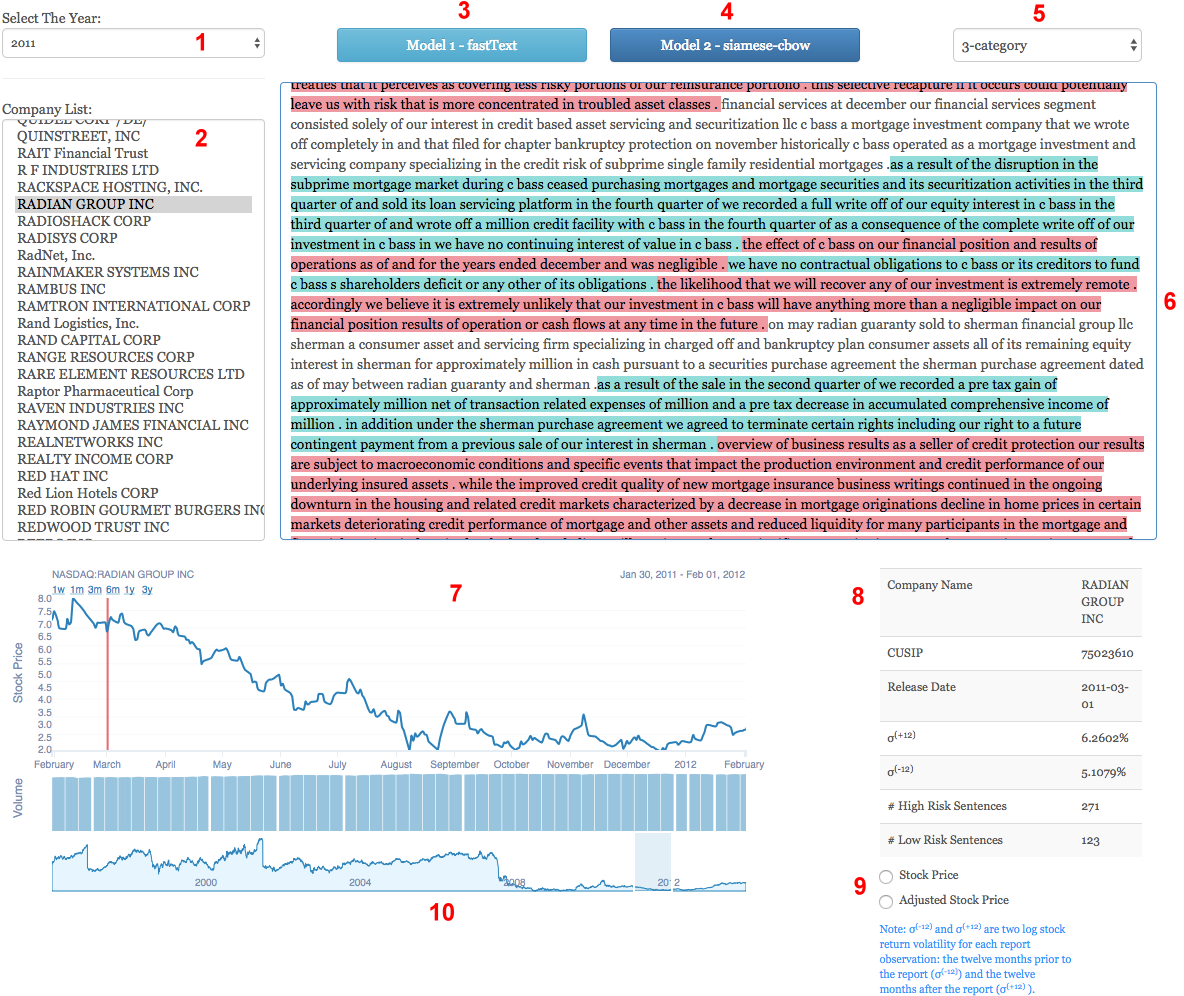
\includegraphics[width=6.6in]{platformdescription.png}
  \caption{The user interface of the RiskFinder system}\label{fig:platformdescription}
\end{figure*}

Figure~\ref{fig:platformdescription} shows the user interface of the
proposed RiskFinder system.
%\begin{enumerate}
%\item
 %The meta data that summarize the basic information about each financial report on Form 10-K, including the basic information about the company that announces this report
 %and some relevant financial measures associated with this report.
%\item
 %The models that highlight and classify the sentences in financial reports
%\item
 %Financial measures visualized through charts to associate with displayed financial reports.
%\item
 %Form 10-K sentiment data set and pre-trained sentences embedding.
%\end{enumerate}
In the system, there are 4 major components for risk detection, the details
of which are provided in the following subsections.

\subsection{Form 10-K Risk-sentiment Dataset}

The first component is the collection of the Form 10-K risk-sentiment dataset.
This work provides the financial risk-sentiment dataset that consists of two
types of data: a set of labeled financial sentences and the pre-trained
sentence embeddings.
There are in total 432 labeled financial sentences in the dataset, which were
selected from the MD\&A\footnote{Management Discussion and Analysis of
Financial Condition and Results of Operations} sections of the 10-K corpus.
When selecting the candidate sentences, we first used the six financial sentiment
lexicons proposed by~\citep{loughran2011liability} to filter sentences and
randomly chose 24 sentences for annotation per year, yielding in total 432
sentences for 18 years (1996 to 2013).
To construct the risk-labeled dataset, eight financial specialists including
accountants, financial analysts and consultants participated in the annotation
task to ensure the quality of the labeling.
In the annotation process, each of the candidate sentences was labeled by
three different annotators, and then the rule of majority was used to determine
the degree of risk of the sentence.
Table~\ref{tab:labelsummary} summarizes the annotation results.  In addition,
the dataset also includes the pre-trained sentence vectors, each of which is a
100-dimension real-valued vector, trained by FastText and Siamese-CBOW on the
10-K corpus and the labeled sentences.\footnote{The dataset is available at
  \url{anonymousurl} upon publication.}

\begin{table}[h]
\centering
\begin{tabular}{ccccc}
  \toprule
Degree of risk & High risk & Neutral & Low risk & Total\\
\midrule
\# of sentences & 138 & 228 & 66 & 432\\
\bottomrule
\end{tabular}
\caption{Labeled sentences}\label{tab:labelsummary}
\end{table}
\vspace*{-0.9cm}
%\begin{figure}[t!]
%\includegraphics[width=3.2in]{dictionary.png}
%\caption{Number of Sentiment Word of Different Categories of Risk in 10-K Sentiment Sentence
%}\label{fig:dictionary}
%\end{figure}

\subsection{The Metadata}

The second component of the proposed system is the metadata of the companies
in the Form 10-K corpus, including basic information on each company such as
the financial report and several financial measures.
A user can first select the year from 1996 to 2013 of the financial reports in
the selection bar (1) of Figure~\ref{fig:platformdescription} and pick the
company documenting the report in that year in the list (2) (e.g., RADIAN GROUP
INC in the figure).
Following the selection, the MD\&A section of the chosen
report\footnote{Only Section 7 MD\&A is used because it contains the most
  important forward-looking statements about the company and is thus related to
  future financial risk~\cite{kogan2009predicting,loughran2011liability}.} is
  then automatically loaded in the window (6).
Then, our system simultaneously displays in table (8) the following metadata which
summarizes the basic information of the corresponding company:
\begin{enumerate}[(a)]
  \item
    the company name;
  \item
    the company's CUSIP number, which facilitates the retrieval of information
    associated with this company from other widely used databases (e.g.,
    Compustat and CRSP\footnote{CRSP is the abbreviation for the Center for
    Research in Security Prices.});
\item
  the report release date;
\item
  the annualized stock return volatilities measured in the twelve-month period
  before and after the announcement of the report (i.e., $\sigma^{(-12)}$ and
  $\sigma^{(+12)}$);
\item
  the number of highlighted risk-related sentences in
  this report.
\end{enumerate}

\subsection{Risk-related Sentence Detection}

\begin{table*}[h]
\centering
\begin{tabular}{lcccccccccc} 
  \toprule
  & \multicolumn{4}{c}{Binary classification} & \multicolumn{6}{c}{Three-class classification}\\ 
\cmidrule(lr){2-5} \cmidrule(lr){6-11}
  & \multicolumn{2}{c}{Siamese-CBOW} & \multicolumn{2}{c}{FastText} & \multicolumn{3}{c}{Siamese-CBOW} & \multicolumn{3}{c}{FastText}\\
\midrule
Accuracy& \multicolumn{2}{c}{0.713} & \multicolumn{2}{c}{0.759} & \multicolumn{3}{c}{0.609} & \multicolumn{3}{c}{0.667} \\ 
\cmidrule(lr){2-11}
& High risk & Low risk  & High risk & Low risk  & High risk & Neutral  & Low risk & High risk & Neutral & Low risk  \\
\cmidrule(lr){2-3}
\cmidrule(lr){4-5}
\cmidrule(lr){6-8}
\cmidrule(lr){9-11}
Precision & 0.600 & 0.736 & 0.640 & 0.806 & 0.632 & 0.619 & 0.400 & 0.655 & 0.686 & 0.571 \\
Recall & 0.324 & 0.898 & 0.571 & 0.848  & 0.429 & 0.813 & 0.182 & 0.679 & 0.729 & 0.364\\
F1-measure& 0.419 & 0.809 & 0.604 & 0.826 & 0.511 & 0.703 & 0.250 & 0.667 & 0.707 & 0.444\\ 
\bottomrule
\end{tabular}
\caption{Performance for risk sentence classification}\label{tab:precision}
\end{table*}

To gauge a company's financial risk given the textual information in its
financial reports on Form 10-K, the proposed system focuses on the
sentence-level investigation into the MD\&A section, which is considered the
part where the firm managements are most likely to reveal information
by the tone they use~\citep{loughran2011liability}.
In our system, two sentence embedding techniques are utilized for
sentence-level textual analyses: Model 1 is FastText which uses a linear
classifier that enables efficient sentence classification and yields
performance on par with other deep learning
classifiers~\citep{bojanowski2016enriching,joulin2016bag}; Model 2 is
Siamese-CBOW, an efficient neural network architecture that obtains
high-quality word embeddings, directly optimized for sentence
representations~\citep{kenter2016siamese}.
Since Siamese-CBOW, the second approach, produces only sentence embedding (by
simply averaging the word embedding of each word in a sentence), we then employ
a logistic regression to construct a classifier.

%\begin{table}
%\centering
%\begin{tabular}{ccc} 
  %\toprule
  %&  \multicolumn{2}{c}{Accuracy}\\
%\cmidrule(lr){2-3}
 %& Binary classification & 3-class classification\\ 
%\midrule
%FastText & 0.759 & 0.667 \\ 
%Siamese-CBOW & 0.713 & 0.609 \\ 
%\bottomrule
%\end{tabular}
%\caption{Summary of labeled data}\label{tab:precision}
%\end{table}

As shown in Figure~\ref{fig:platformdescription}, by clicking button (3) or
(4), users use Model 1 or 2 to classify the sentences in the MD\&A section
for a certain financial report into three parts: those highlighted red
representing high-risk sentences; those highlighted green representing low-risk
ones; and others representing those irrelevant to financial risk.
The three-class classification task can be reduced to a binary one through the
selection bar (5): high-risk sentences in red and others in white.
Table~\ref{tab:precision} tabulates the performance of both classification
tasks tested on the 87 sentences in terms of accuracy, precision, recall, and
F1-measure.\footnote{The 432
sentences are split into the training data and the testing data with 435 and 87
sentences, respectively.} Note that for binary classification, we consider
both neutral and low-risk sentences as irrelevant to financial risk.
Finally, the numbers of highlighted risk-related sentences are summarized in
table (8) of Figure~\ref{fig:platformdescription}.

\subsection{Visualization for Financial Measures}

Our system attempts to facilitate the analysis of textual information and
capture more insight into the financial risk associated with the announcement of
each financial report.
Therefore, in addition to highlighting the risk-related sentences, our system
also displays time-aligned quantitative information for comparison purposes,
such as historical prices and trading volumes of the selected company's stock,
as shown in the chart (7) of Figure~\ref{fig:platformdescription}.
In particular, the release date of the report is highlighted through a red
vertical line in the chart; users adjust the window (10) to show the
corresponding quantitative information for a certain period.
Note that two types of historical stock prices are provided in the proposed
system: the original stock prices and those adjusted due to stock splits and
dividend payouts; the mode can be altered through (9).

\section{Case Study}\label{sec:case}

%Building an information system based on the sentence-level analysis is
%essential because most of the financial keywords are context-sensitive and thus
%focusing the content analysis merely on word level probably makes the
%inferences bias against the true results.

\begin{figure}[tbh]
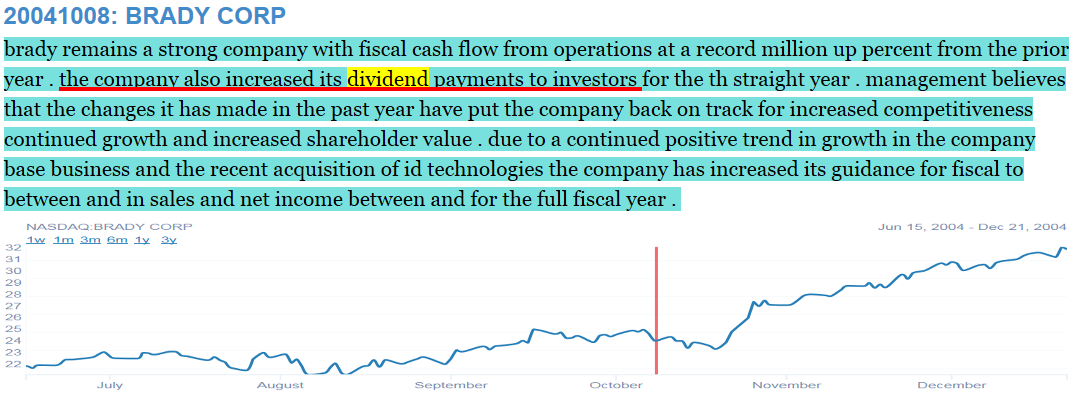
\includegraphics[height=1.65in, width=3.5in]{dividend_positive.png}
\caption{A low-risk word
in a low-risk sentence} \label{fig:dividend_lowrisksentence}
\end{figure}

\begin{figure}[tbh]
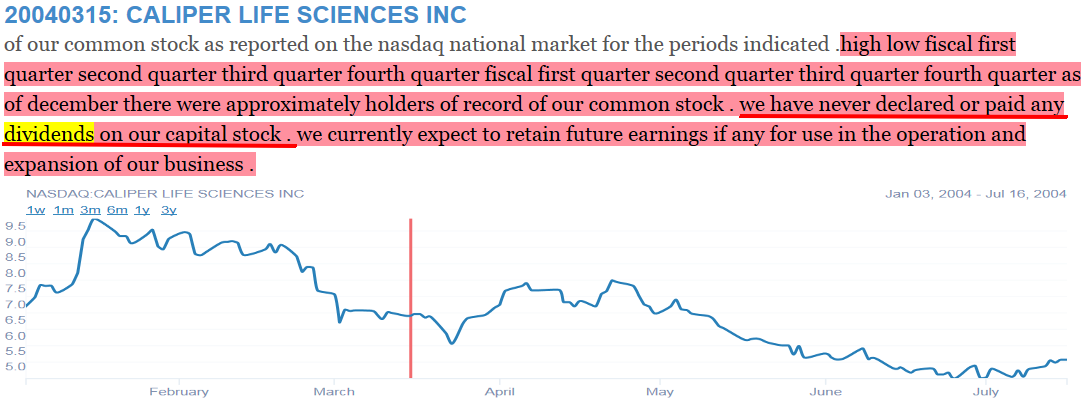
\includegraphics[height=1.65in, width=3.5in]{dividend_negative.png}
\caption{A low-risk word
in a high-risk sentence}\label{fig:dividend_highrisksentence}
\end{figure}

Here we showcase some interesting cases to demonstrate the need to
conduct sentence-level analysis on finance textual information and the
usability of the proposed system.
The word ``dividend'' displayed as follows is a notable example.
According to financial literature such as~\cite{denis2008firms}, dividend is
empirically treated as a low-risk word because companies with the propensity to pay
dividends are assumed to be profitable ones.
Figure~\ref{fig:dividend_lowrisksentence} shows Brady Corp.'s
stock prices trend upward after the announcement of its year 2004 financial
report stating that ``the company also increased its dividend payments to
investors \ldots.''
However, Figure~\ref{fig:dividend_highrisksentence} exhibits an opposite case
from the sentence-level point of view, because another company, Caliper Life
Science Inc.\ states that ``we have never declared or paid any dividends on our
capital stock'' in its year 2004 report.

Several similar cases can also be founded via the proposed RiskFinder system.
For example, from the sentence-level analysis point of view, 
the low-risk word ``profit'' (discovered in the study 
of~\cite{tsai2017risk}) may refer to either ``increase in gross profits'' or
``reduction in gross profits'';
the high-risk word ``deficit'' sometimes reveals positive signals such as
``reducing the company working capital deficit and increase liquidity
$\ldots$''\footnote{ For example, see Mallon Resources Corp.'s
annual report for 1996.} or the usual negative ones like ``the gross deficit incurred
resulted from costs of products $\ldots$.''

\section{Conclusions}\label{sec:conclusion}

In this paper we introduce RiskFinder, a web-based information system that
broadens the textual analysis of financial reports from the word level to the
sentence level.
This extension is essential especially for the analysis of financial keywords because
most of these words are context-sensitive.
Built on financial reports in the 10-K Corpus with a set of labeled sentences about
financial risk, this proposed system applies two sentence embedding techniques --- 
FastText and Siamese-CBOW --- to automatically classify the risk-related sentences
in those reports as being positively, negatively or
insignificantly related to financial risk.
For comparison purposes, the system even displays the time-aligned relevant
quantitative information to visualize the financial risk associated with the
announcement of each report.
This system greatly facilitates case studies in the finance field for
scholars and can be of great help for practitioners in capturing meaningful
insight within large amounts of textual information in finance from the 
sentence-level point of view.
The system is now online available at~\url{https://cfda.csie.org/RiskFinder/}.

This work is a preliminary study, the purpose of which is to demonstrate the
importance of sentence-level analysis and the integration of soft and hard
information in finance. 
Therefore, in the future, we will continue to extend the system, with an emphasis
on incorporating more state-of-the-art learning algorithms or developing new
algorithms to better detect risk-related sentences.
%\subsection{Theorem-like Constructs}
%
%Other common constructs that may occur in your article are the forms
%for logical constructs like theorems, axioms, corollaries and proofs.
%ACM uses two types of these constructs:  theorem-like and
%definition-like.
%
%Here is a theorem:
%\begin{theorem}
%  Let $f$ be continuous on $[a,b]$.  If $G$ is
%  an antiderivative for $f$ on $[a,b]$, then
%  \begin{displaymath}
%    \int^b_af(t)\,dt = G(b) - G(a).
%  \end{displaymath}
%\end{theorem}
%
%Here is a definition:
%\begin{definition}
%  If $z$ is irrational, then by $e^z$ we mean the
%  unique number that has
%  logarithm $z$:
%  \begin{displaymath}
%    \log e^z = z.
%  \end{displaymath}
%\end{definition}
%
%The pre-defined theorem-like constructs are \textbf{theorem},
%\textbf{conjecture}, \textbf{proposition}, \textbf{lemma} and
%\textbf{corollary}.  The pre-defined de\-fi\-ni\-ti\-on-like constructs are
%\textbf{example} and \textbf{definition}.  You can add your own
%constructs using the \textsl{amsthm} interface~\cite{Amsthm15}.  The
%styles used in the \verb|\theoremstyle| command are \textbf{acmplain}
%and \textbf{acmdefinition}.
%
%Another construct is \textbf{proof}, for example,
%
%\begin{proof}
%  Suppose on the contrary there exists a real number $L$ such that
%  \begin{displaymath}
%    \lim_{x\rightarrow\infty} \frac{f(x)}{g(x)} = L.
%  \end{displaymath}
%  Then
%  \begin{displaymath}
%    l=\lim_{x\rightarrow c} f(x)
%    = \lim_{x\rightarrow c}
%    \left[ g{x} \cdot \frac{f(x)}{g(x)} \right ]
%    = \lim_{x\rightarrow c} g(x) \cdot \lim_{x\rightarrow c}
%    \frac{f(x)}{g(x)} = 0\cdot L = 0,
%  \end{displaymath}
%  which contradicts our assumption that $l\neq 0$.
%\end{proof}


%\appendix
%%Appendix A
%\section{Headings in Appendices}
%The rules about hierarchical headings discussed above for
%the body of the article are different in the appendices.
%In the \textbf{appendix} environment, the command
%\textbf{section} is used to
%indicate the start of each Appendix, with alphabetic order
%designation (i.e., the first is A, the second B, etc.) and
%a title (if you include one).  So, if you need
%hierarchical structure
%\textit{within} an Appendix, start with \textbf{subsection} as the
%highest level. Here is an outline of the body of this
%document in Appendix-appropriate form:
%\subsection{Introduction}
%\subsection{The Body of the Paper}
%\subsubsection{Type Changes and  Special Characters}
%\subsubsection{Math Equations}
%\paragraph{Inline (In-text) Equations}
%\paragraph{Display Equations}
%\subsubsection{Citations}
%\subsubsection{Tables}
%\subsubsection{Figures}
%\subsubsection{Theorem-like Constructs}
%\subsubsection*{A Caveat for the \TeX\ Expert}
%\subsection{Conclusions}
%\subsection{References}
%Generated by bibtex from your \texttt{.bib} file.  Run latex,
%then bibtex, then latex twice (to resolve references)
%to create the \texttt{.bbl} file.  Insert that \texttt{.bbl}
%file into the \texttt{.tex} source file and comment out
%the command \texttt{{\char'134}thebibliography}.
%% This next section command marks the start of
%% Appendix B, and does not continue the present hierarchy
%\section{More Help for the Hardy}
%
%Of course, reading the source code is always useful.  The file
%\path{acmart.pdf} contains both the user guide and the commented
%code.

%\begin{acks}
  %The authors would like to thank Dr. Yuhua Li for providing the
%  matlab code of  the \textit{BEPS} method.
%
%  The authors would also like to thank the anonymous referees for
%  their valuable comments and helpful suggestions. The work is
%  supported by the \grantsponsor{GS501100001809}{National Natural
%    Science Foundation of
%    China}{http://dx.doi.org/10.13039/501100001809} under Grant
%  No.:~\grantnum{GS501100001809}{61273304}
%  and~\grantnum[http://www.nnsf.cn/youngscientsts]{GS501100001809}{Young
%    Scientsts' Support Program}.
%\end{acks}

\bibliographystyle{ACM-Reference-Format}
\bibliography{paper}

\end{document}
